\section{User interface}

The main chess interface will be an 8x8 board with alternating colors. On the right side of the board there will 
be a console with the players name, signaling whose turn it is. Below the names will be a move history showing all prior moves made during the current game. At the bottom of this menu will be a submit button which the player must
click to signal the end of his turn and to start the move validation.

While playing, the players will click on the chess piece they wish to move and then click on the location they wish to move it to. If the player is attempting a special move like castling, they would click on the first piece and then its final location followed by the second piece and its final location before clicking submit. There will also be a 'game info' button at the bottom: when clicked, it will show a 'popover' style window above the board to display information about the game, credit Siberia Software with its development and thank anyone else involved, display logos of company and game, and show or link to any other relevant information (links should open in a new window in order to not disrupt gameplay). Also, any error messages will be shown as Windows-type dialog boxes, also above the board the same way as the informational pop-over.
\begin{figure}[H]
   \centering
   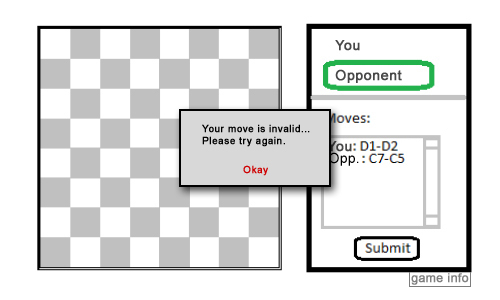
\includegraphics[scale=1.0]{screenshot7.jpg}
   \caption{Example Screen}
  \end{figure}
  %\FloatBarrier

\begin{figure}[H]
   \centering
   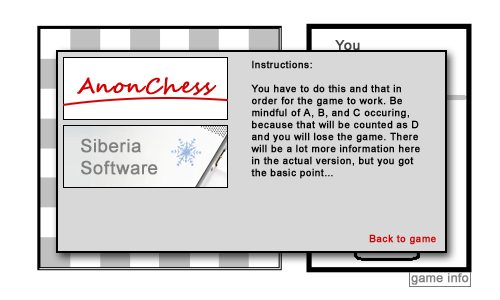
\includegraphics[scale=1.0]{screenshot4.jpg}
   \caption{Example Screen}
  \end{figure}
  %\FloatBarrier

\begin{figure}[H]
   \centering
   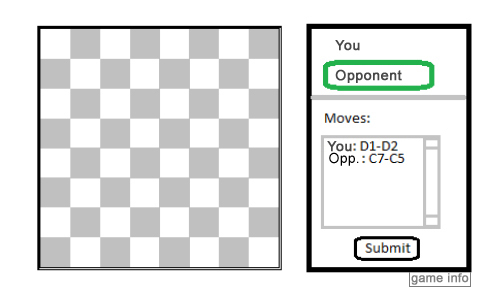
\includegraphics[scale=1.0]{screenshot6.jpg}
   \caption{Example Screen}
  \end{figure}
  %\FloatBarrier

